\part{Skeletal animation}
\frame{\partpage}

\begin{frame}{Rigging}
	\begin{columns}
		\begin{column}{0.4\textwidth}
			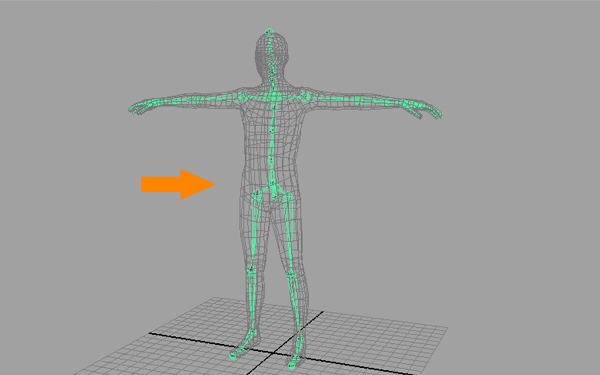
\includegraphics[width=\textwidth]{human_rig}
		\end{column}
		\begin{column}{0.58\textwidth}
			\begin{itemize}
				\pause\item A \textbf{skeleton} is composed of \textbf{bones}
				\pause\item Arranged in a \textbf{hierarchy}
				\pause\item Each bone is essentially just a \textbf{transformation}
					\begin{itemize}
						\pause\item Usually just rotation around a pivot point
						\pause\item 3D modelling software often represents bones as lines from parent bone to child bone
					\end{itemize}
			\end{itemize}
		\end{column}
	\end{columns}
\end{frame}

\begin{frame}{Bone weights}
	\begin{columns}
		\begin{column}{0.4\textwidth}
			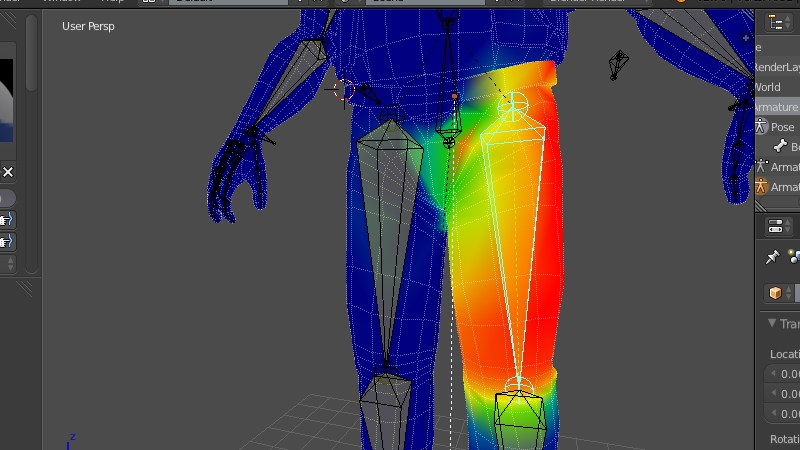
\includegraphics[width=\textwidth]{bone_weights}
		\end{column}
		\begin{column}{0.58\textwidth}
			\begin{itemize}
				\pause\item Each vertex in the model has a list of \textbf{bone weights}
				\pause\item Usually ``painted'' onto the model by the 3D artist
				\pause\item Weights specify how much each vertex is affected by each bone's transformation
			\end{itemize}
		\end{column}
	\end{columns}
\end{frame}

\begin{frame}{Skinning}
	\begin{itemize}
		\pause\item The character is animated by changing the bone transformations
		\pause\item \textbf{Skinning} is the process of applying these transformations to the vertices of the model
			according to the bone weights
		\pause\item Generally handled by a \textbf{vertex shader}
	\end{itemize}
\end{frame}

\begin{frame}{Keyframe animation}
	\begin{itemize}
		\pause\item Most basic form of skeletal animation: specify bone transformations for each frame of animation
		\pause\item ... or just for \textbf{keyframes} and interpolate between them
		\pause\item Keyframes set up by an animator, through motion capture, or a combination of the two
		\pause\item More advanced: can \textbf{blend} animations
			\begin{itemize}
				\pause\item E.g.\ blend between walking and running
				\pause\item E.g.\ bottom half plays ``walk'' animation, top half plays ``fire weapon'' animation
			\end{itemize}
	\end{itemize}
\end{frame}

\begin{frame}{Forward kinematics (FK)}
	\begin{columns}
		\begin{column}{0.4\textwidth}
			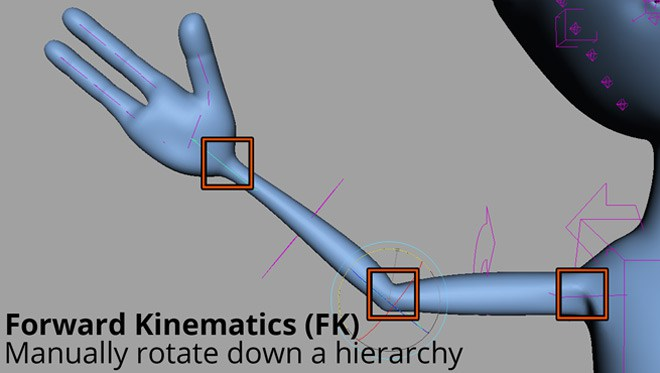
\includegraphics[width=\textwidth]{forward_kinematics}
		\end{column}
		\begin{column}{0.58\textwidth}
			\begin{itemize}
				\pause\item Bone transformations are set \textbf{explicitly}
				\pause\item Children are affected by parent transformations,
					e.g.\ if upper arm rotates, lower arm rotates with it
			\end{itemize}
		\end{column}
	\end{columns}
\end{frame}

\begin{frame}{Inverse kinematics (IK)}
	\begin{columns}
		\begin{column}{0.4\textwidth}
			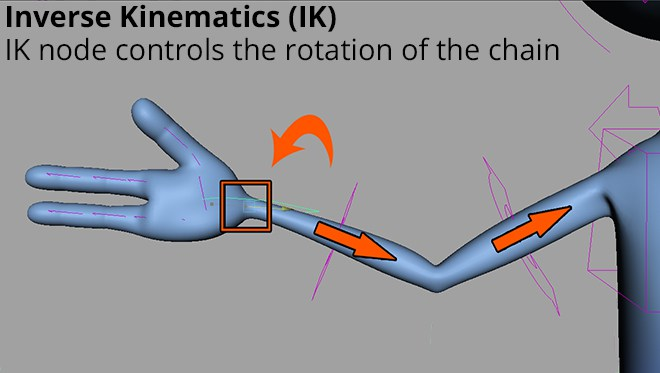
\includegraphics[width=\textwidth]{inverse_kinematics}
		\end{column}
		\begin{column}{0.58\textwidth}
			\begin{itemize}
				\pause\item Bone transformations are calculated to reach a \textbf{target}
				\pause\item E.g.\ we want character's hand to touch an object; IK calculates rotations of upper and lower arm to achieve this
					subject to constraints
			\end{itemize}
		\end{column}
	\end{columns}
\end{frame}

\begin{frame}{The most common use for IK}
	\begin{center}
		\pause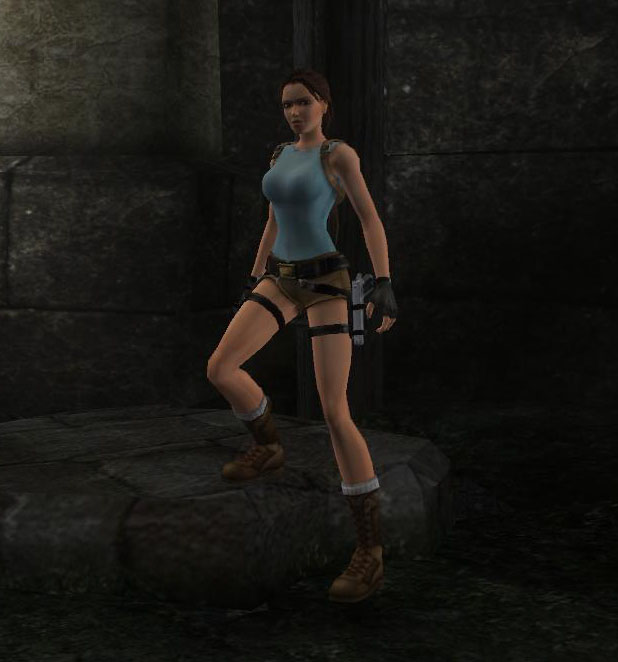
\includegraphics[height=0.4\textheight]{ik_feet3} \quad
		\pause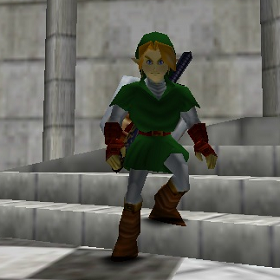
\includegraphics[height=0.4\textheight]{ik_feet2}
		
		\pause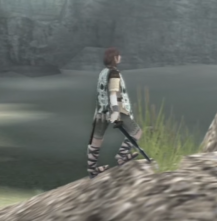
\includegraphics[height=0.4\textheight]{ik_feet4} \quad
		\pause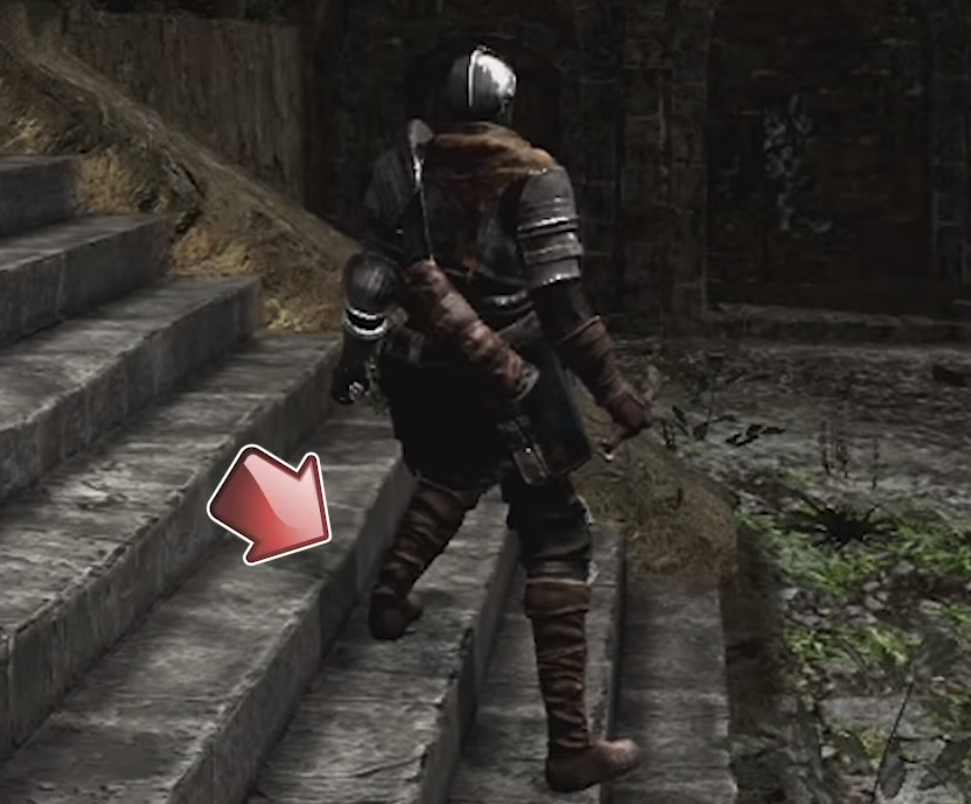
\includegraphics[height=0.4\textheight]{ik_feet}
	\end{center}
\end{frame}

\begin{frame}{Ragdolls}
	\begin{columns}
		\begin{column}{0.4\textwidth}
			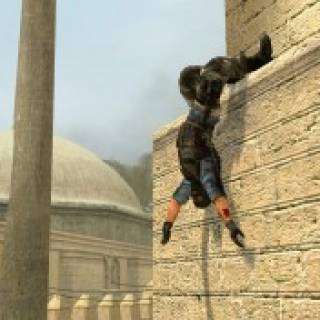
\includegraphics[width=\textwidth]{ragdoll}
		\end{column}
		\begin{column}{0.58\textwidth}
			\begin{itemize}
				\pause\item Attach a \textbf{rigid body} to each bone and run a \textbf{physics simulation}
				\pause\item Often used for death animations
			\end{itemize}
		\end{column}
	\end{columns}
\end{frame}

\begin{frame}{Procedural animation}
	\begin{itemize}
		\pause\item Many games mix some or all of keyframe animation, IK, and physics simulation
		\pause\item \url{https://www.youtube.com/watch?v=JEzxDbIK2Yk}
		\pause\item \url{https://www.youtube.com/watch?v=UQdkkmP7amI}
	\end{itemize}
\end{frame}
